\documentclass{article}
\usepackage{stackengine}
%\usepackage[utf8]{inputenc}
\usepackage[T1]{fontenc}
\usepackage{amsmath}
\usepackage{amsfonts}
\usepackage{graphicx}
\usepackage{pbsi}
\usepackage{lmodern}
%\usepackage{tgbonum}
\usepackage[a4paper]{geometry}
\usepackage{pdflscape}
\usepackage[dvipsnames, svgnames]{xcolor}
\usepackage[pages=some]{background}
\usepackage{tikz}
\usetikzlibrary{math} 
\usetikzlibrary{automata,positioning}
\usetikzlibrary[decorations.text]
\usetikzlibrary{arrows.meta} % LATEX and plain TEX when using Tik Z
%\usetikzlibrary[automata]
\usetikzlibrary{calc}

\newcommand\BackImage[2][scale=1]{%
\BgThispage
\backgroundsetup{
scale=1,
angle=0,
opacity=1,  %% adjust
contents={\includegraphics[width=\paperwidth,height=\paperheight]{#2}}
%contents={\includegraphics[#1]{#2}}
}
}

\newcommand*{\vertchar}[2][0pt]{%
  \tikz[
    inner sep=1pt,
    shorten >=-.15ex,
    shorten <=-.15ex,
    line cap=round,
    baseline=(c.base),
  ]\draw
    (0,0) node (c) {#2}
    ($(c.north)+(#1,0)$) -- ($(c.north)+(#1,0)$);%
}


\makeatletter
\newcommand{\dotr}[1]{%
  \mathpalette\@dotr{#1}%
}

\newcommand*{\@dotr}[2]{%
  % #1: math style (\displaystyle, ..., \scriptscriptstyle)
  % #2: argument of \dotr
  \sbox0{$\m@th#1#2$}%
  \usebox{0}%
  % simulating a superscript
  %\raisebox{\dimexpr\ht0-\height}{$\m@th#1\addvbuffer[-1ex 0.9ex]{.}}%
  \raisebox{3.5pt}{$\m@th#1\@smallbullet#1\bullet$}%
  \kern\scriptspace
}
\newcommand*{\@smallbullet}[2]{%
  \scalebox{.3}{$\m@th#1#2$}%
}
\makeatother
    
\newcommand*{\siin}[1]{\stackinset{c}{}{b}{5.5pt}{\small\ttfamily\char'15}{#1}}
\newcommand*{\nn}{\textsuperscript{n}}

\newcommand*{\pehin}[1]{\stackinset{c}{}{b}{5.5pt}{\small\ttfamily\char'15}{#1}}
\newcommand*{\dtr}{\raisebox{3.5pt}{$\scalebox{.3}{$\bullet$}$}}
\newcommand*{\dtrh}{\raisebox{5pt}{$\scalebox{.3}{$\bullet$}$}}

\setlength{\footskip}{100pt}


\begin{document}

\hspace*{-25mm}
\resizebox{18cm}{!} {
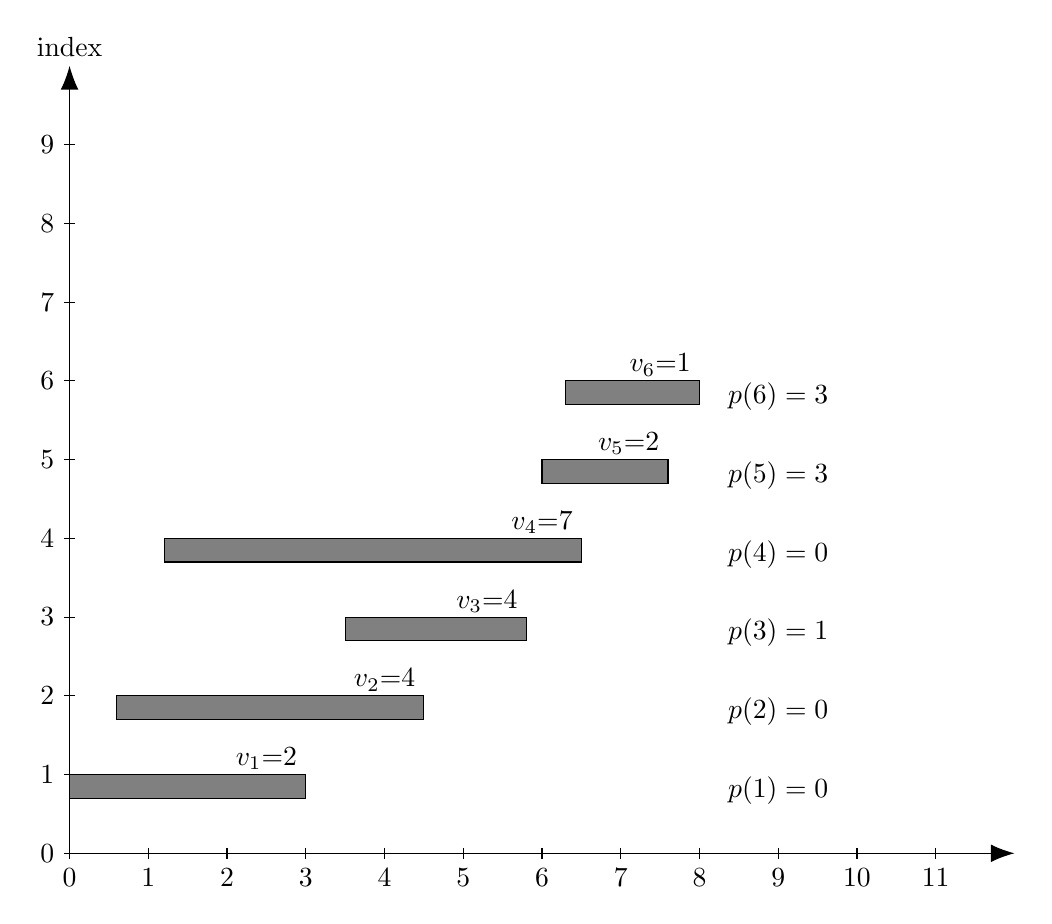
\begin{tikzpicture} 
\foreach \x in {0,...,11}
   \draw (\x cm,2pt) -- (\x cm,-2pt) node[anchor=north] {$\x$};
\foreach \y in {0,...,9}
    \draw (2pt,\y cm) -- (-2pt,\y cm) node[anchor=east] {$\y$};
\draw[[-{Latex[length=3mm]}] (0,0) -- (12,0) node [anchor= north]{};
\draw[[-{Latex[length=3mm]}] (0,0) -- (0,10) node [anchor= south] {index};

\filldraw [fill=gray] (0,0.7) rectangle (3,1);
\path (2.5, 1.2) node {$v_1$=2};
\filldraw [fill=gray] (0.6,1.7) rectangle (4.5,2);
\path (4, 2.2) node {$v_2$=4};
\filldraw [fill=gray] (3.5,2.7) rectangle (5.8,3);
\path (5.3, 3.2) node {$v_3$=4};
\filldraw [fill=gray] (1.2,3.7 ) rectangle (6.5,4);
 \path (6, 4.2) node {$v_4$=7};
\filldraw [fill=gray] (6 ,4.7) rectangle (7.6, 5);
\path (7.1,5.2) node {$v_5$=2};
\filldraw [fill=gray] (6.3,5.7) rectangle (8,6);
\path (7.5,6.2) node {$v_6$=1};
 
\path (9, 0.8) node {$p(1)=0$};
\path (9, 1.8) node {$p(2)=0$};
\path (9, 2.8) node {$p(3)=1$};
\path (9, 3.8) node {$p(4)=0$};
\path (9, 4.8) node {$p(5)=3$};
\path (9, 5.8) node {$p(6)=3$};

\end{tikzpicture}
}
\vspace*{5mm} \newline
\hspace*{30mm}
{\LARGE The Weighted Interval Problem};


\newpage
\hspace*{-25mm}
\resizebox{18cm}{!} {
\begin{tikzpicture} 
\foreach \x in {0,...,11}
   \draw (\x cm,2pt) -- (\x cm,-2pt) node[anchor=north] {$\x$};
\foreach \y in {0,...,9}
    \draw (2pt,\y cm) -- (-2pt,\y cm) node[anchor=east] {$\y$};
\draw[[-{Latex[length=3mm]}] (0,0) -- (12,0) node [anchor= north]{};
\draw[[-{Latex[length=3mm]}] (0,0) -- (0,10) node [anchor= south] {index};

\path (6.5,8) node (c1) {\small OPT(6)};
\path (5,7) node (c2) {\small OPT(5)};
\path (8,7) node (c3) {\small OPT(3)};
\path (4, 6) node (c4) {\small OPT(4)};
\path (5.5, 6) node (c5) {\small OPT(3)};
\path (7.5, 6) node (c6) {\small OPT(2)};
\path (9, 6) node (c7) {\small OPT(1)};
\path (3,4.5) node (c8) {\small OPT(3)};
\path (4.5,4.5) node (c9) {\small OPT(2)};
\path (6,4.5) node (c10) {\small OPT(1)};
\path (7.5,4.5) node (c11) {\small OPT(1)};
\path (1.5,3) node (c12) {\small OPT(2)};
\path (3,3) node (c13) {\small OPT(1)};
\path (4.5,3) node (c14) {\small OPT(1)};
\path (1.5,1.5) node (c15) {\small OPT(1)};


\draw[[-{Latex[length=2mm]}] (c1) to (c2);
\draw[[-{Latex[length=2mm]}] (c1) to (c3);
\draw[[-{Latex[length=2mm]}] (c2) to (c4);
\draw[[-{Latex[length=2mm]}] (c2) to (c5);
\draw[[-{Latex[length=2mm]}] (c3) to (c6);
\draw[[-{Latex[length=2mm]}] (c3) to (c7);
\draw[[-{Latex[length=2mm]}] (c4) to (c8);
\draw[[-{Latex[length=2mm]}] (c5) to (c9);
\draw[[-{Latex[length=2mm]}] (c5) to (c10);
\draw[[-{Latex[length=2mm]}] (c6) to (c11);
\draw[[-{Latex[length=2mm]}] (c8) to (c12);
\draw[[-{Latex[length=2mm]}] (c8) to (c13);
\draw[[-{Latex[length=2mm]}] (c9) to (c14);
\draw[[-{Latex[length=2mm]}] (c12) to (c15);

\path (6.5, 9) node {Tree of Calls};

\end{tikzpicture}
}
\vspace*{5mm} \newline
\hspace*{30mm}
{\LARGE The Weighted Interval Problem} \newline
\vspace*{1mm} \newline
\hspace*{-10mm} \parbox[t][20mm][l] {135mm} {
\rule[1mm]{120mm}{1pt} \newline
{\large \ttfamily Compute-Opt($j$)} \newline
\hspace*{2mm} {\large \ttfamily If $j=0$ then} \newline
\hspace*{5mm} {\large \ttfamily Return $0$} \newline
\hspace*{2mm} {\large \ttfamily Else} \newline
\hspace*{5mm} {\large \ttfamily Return max($v_j$+Compute-Opt(p($j$)), Compute-Opt($j-1$))} \newline
\hspace*{2mm}  {\large \ttfamily Endif} \newline
\rule[-1mm]{120mm}{1pt} \newline
}
\end{document}